\section{Strumenti di lavoro}
\subsection{Coordinamento}
\subsubsection{Strumento per la gestione del progetto}
Al fine di gestire rigorosamente lo sviluppo del progetto il team \gruppo{} ha adottato l'utilizzo del software \textit{TeamWorkPM} (\href{http://www.teamwork.com}{www.teamwork.com}), tale strumento fornisce le seguenti funzionalità:

\begin{itemize}
\item Creazione di \textit{ticket\ped{G}}, \textit{milestone\ped{G}} e liste di attività;
\item Creazione ed assegnazione di attività;
\item Calendario di progetto;
\item \textit{Report} automatico giornaliero delle attività svolte ed in ritardo inviato tramite \textit{e-mail};
\item Gestione dei ruoli;
\item Generazione di grafici \textit{Gantt\ped{G}} a partire dalle \textit{task-list};
\item Monitoraggio dei tempi;
\item Registro dei rischi.
\end{itemize}

Sono stati valutati altri software come ad esempio \textit{Redmine}, il quale fu ritenuto quasi altrettanto completo ed intuitivo. Tuttavia si è optato per \textit{TeamWorkPM} data la sua estrema semplicità di utilizzo.\\
Il \textit{Responsabile di Progetto} per garantire il regolare svolgimento delle attività dovrà necessariamente verificare con cadenza giornaliera se sono presenti \textit{ticket} scaduti e non ancora completati, nel caso citato infatti sarà obbligato a richiedere informazioni (o in caso di ritardi gravi convocare l'interessato) circa la causa del ritardo.\\
Infine, il \textit{Responsabile di Progetto} dovrà tenere nota che l'assegnazione di \textit{ticket} la cui scadenza è prevista per il giorno successivo può avvenire solo se il lavoro da svolgere non supera le 2 ore lavorative.

\subsubsection{Strumento di versionamento}
Di pressoché fondamentale importanza è stata la definizione di un ambiente ordinato in cui organizzare e mantenere tutti i \textit{file} che attraversano il ciclo di vita, per questa ragione è stato scelto di avvalersi di un \textit{repository}. 

\paragraph{GitHub}
Come sistema di controllo di versione è stato adottato il software \textit{GitHub\ped{G}}, i pregi di questo strumento vengono qui di seguito riportati:
\begin{itemize}
\item Molto reattivo;
\item Design semplice; 
\item \textit{Software} gratuito.
\end{itemize}

\paragraph{Struttura repository}
L'indirizzo di \textbf{root\ped{G}} del \textit{repository} contenente tutta la documentazione è:
\begin{center}
\href{https://github.com/Dquaglio/Sirius}{https://github.com/Dquaglio/Sirius}
\end{center}

Ogni documento presente sarà contenuto in una sotto cartella del \textit{master branch\ped{G}} nominata come il nome del documento stesso.
All'interno della cartella potranno essere contenuti solamente \textit{file.tex}, per la visualizzazione del relativo \textit{pdf\ped{G}} sarà necessario scaricarli e compilarli, assicurandosi di avere l'ultima versione del modello disponibile.
\begin{center}
\textbf{modello.git}: \href{https://github.com/Dquaglio/Sirius/tree/master/modello.git}{https://github.com/Dquaglio/Sirius/tree/master/modello.git}
\end{center}

conterrà il \textit{template} \LaTeX, le \textit{macro} e gli script aggiornati all'ultima versione disponibile.
\\
\\
Il \textit{master branch} è stato quindi suddiviso seguendo questa struttura:
\begin{figure}
\centering
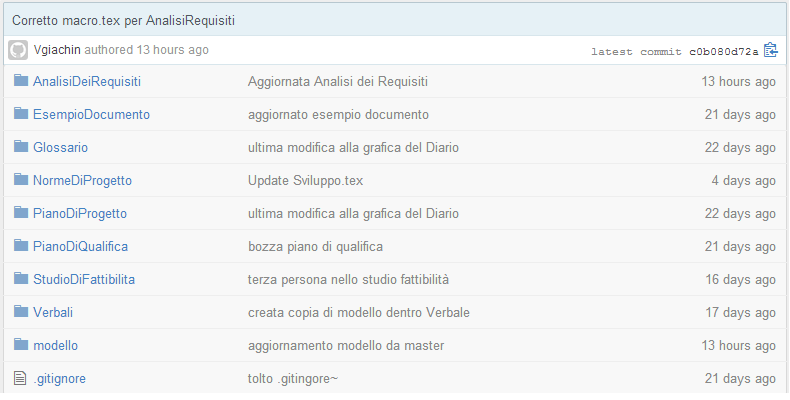
\includegraphics[width= %
\linewidth]{immaginiNDP/repository}
\caption[]{Struttura master branch.}
\label{fig:repository}
\end{figure}
A scopo puramente dimostrativo è stato creato l'esempio di un documento formale del gruppo \gruppo, contenuto nella cartella: "EsempioDocumento", questa scelta è stata fatta per illustrare la struttura generale che deve preservare qualsiasi documento (sezione 5.4, Struttura documentazione).
Per sfruttare il parallelismo nello sviluppo di uno stesso documento sono stati creati appositamente dei  \textit{branch} denominati con il nome dei membri del gruppo, i documenti  \textit{baseline\ped{G}} invece saranno contenuti solamente nel \textit{master branch}. Il \textit{merge\ped{G}} con il ramo \textit{master} avviene quindi solamente dopo la terminazione dell'attività di verifica di un documento.

\subsubsection{Strumenti per la condivisione file}
Per gestire efficientemente la condivisione dei file intra-gruppo a supporto dello strumento di \textbf{Git} è stato scelto l'utilizzo di: Google Drive, un servizio \textit{web} di \textit{storage} e sincronizzazione \textit{online} che dovrebbe facilitare la condivisione e fornire una base d'appoggio secondaria ed informale per alcuni file che non necessitano versionamento.
L'utilizzo di \textit{Google Drive} e' limitato ai documenti che:
\begin{itemize}
\item Non necessitano di versionamento;
\item Necessitano di essere acceduti velocemente tramite \textit{web};
\end{itemize}

\subsection{Pianificazione}

Per l'attività di pianificazione del progetto nonché gestione delle risorse è stato adottato il software GanttProject, software open source basato su piattaforma Java. Qui di seguito vengono elencate le principali caratteristiche che hanno portato alla scelta di questo strumento:
\begin{itemize}
\item Portabilità, essendo un software basato su Java;
\item Open-source\ped{G};
\item Compatibile con MicrosoftProject;
\item Può generare grafici Work Breakdown Structure (WBS\ped{G});
\item Fornisce la possibilità di creare grafici di Gantt\ped{G};
\item Può generare grafici Program Evalutation and Review Tecnique (PERT\ped{G});
\item In grado di gestire e generare grafici delle risorse assegnate.
\end{itemize}
\subsection{Strumenti per la documentazione}
\subsubsection{LaTeX}
Per la stesura dei documenti il team \gruppo{} ha deciso di adottare il linguaggio di markup\ped{G} \LaTeX la scelta è stata effettuata prevalentemente per le seguenti ragioni:
\begin{itemize}
\item Facilità di separazione tra contenuto
e formattazione;
\item Possibilità di definire macro ed incorporare scripts;
\item Software open source;
\item Grande quantità di pacchetti disponibili, possibilità quindi di implementare semplicemente le funzionalità comuni.
\end{itemize}
Gli altri software valutati (Open office, Microsoft Office, Google Docs) non erano in grado di fornire il più delle sopracitate funzionalità, di conseguenza sono stati scartati. Inoltre come editor è consigliato ma non obbligato l'uso di TeXstudio.

\subsubsection{Macro}
Al fine di velocizzare il lavoro di stesura documenti, il team \gruppo{} ha deciso di creare delle apposite macro, qui vengono riportate le principali assieme ad una breve spiegazione delle loro funzionalità:
\begin{itemize}
\item \verb+\+gruppo riporta il nome del team \gruppo;
\item \verb+\+progetto riporta il nome del progetto: \progetto;
\item \verb+\+lastversion+sigla-del-documento riporta il nome del documento che appare in sigla (NDP, AR, etc..) aggiornato alla versione più recente.

\end{itemize}
\subsubsection{Scripts}
Al fine di implementare una funzionalità quale l'inserimento automatico dei pedici in tutte le parole dei documenti formali che comparivano anche nel glossario, è stato creato uno script apposito in Pyton\ped{G}. Tale script può essere essere eseguito solamente con una versione di Pyton non superiore alla 2.7.6.
Per il corretto funzionamento dello script il glossario è stato organizzato tramite tag \LaTeX elemento{"parola del glossario"}, la definizione è riportata a capo-riga rispetto alla suddetta parola. 

\subsubsection{Correttezza}
\paragraph{Correttezza ortografica}
Per evitare di compiere errori di tipo ortografico devono essere adottate due precauzioni:
\begin{itemize}
\item Verifica delle parole durante la stesura stessa del documento tramite lo spell checker\ped{G} di TeXstudio;
\item Verifica finale tramite lo spell checker Aspell.
\end{itemize}
Lo spell checker di TeXstudio è una sua feature\ped{G} molto utile che sfrutta dizionari Open Office per sottolineare eventuali parole scorrette, dizionari sufficientemente completi che assicurano quindi un grado piuttosto elevato di correttezza già durante la stesura del testo. \\
Al fine poi di assicurarsi il massimo grado possibile di correttezza viene effettuata una verifica ulteriore tramite il software open source GNU Aspell
(\href{http://www.aspell.net/}{www.aspell.net}).
 
\paragraph{Lista controllo errori}
Il team ha stilato una lista di controllo al fine di riassumere gli errori più ricorrenti in ogni documento, i suddetti saranno catalogati e descritti nella seguente sezione.
\paragraph{Errori stilistici e di punteggiatura}
I principali errori rilevati sono i seguenti:
\begin{itemize}
\item Le figure di rilievo non vengono scritte in corsivo;
\item Negli elenchi puntati la prima parola non compare con la prima lettera maiuscola;
\item Negli elenchi puntati alcuni elementi centrali non terminano con un punto e virgola ma con un punto fermo;
\item Alcune date vengono erroneamente scritte senza seguire lo standard \textbf{ISO G 8601:2004};
\item La parola LaTeX compare senza l'utilizzo del comando \verb+\+LaTeX (\LaTeX).
\end{itemize}
\paragraph{Errori ortografici e di sintassi}
\begin{itemize}
\item La è accentata compare (erroneamente) come una e apostrofata;
\item Utilizzando le seguenti macro \verb+\+gruppo e \verb+\+progetto, le quali scrivono testualmente e rispettivamente il nome del team ed il nome del capitolato, non compaiono separate dalla parola successiva, anche se la spaziatura è presente;
\item Non viene utilizzata (erroneamente) la terza persona per la stesura dei documenti.
\end{itemize}
\subsubsection{UML}
Per la modellazione dei diagrammi User Case (UC\ped{G}) sono stati presi in considerazione tre editor: Dia, Microsoft Visio, Astah. Infine il team ha optato per adottare Astah come strumento definitivo in quanto si tratta di un software open source, con supporto di Unified Modeling Language (UML\ped{G}) 2.x  e secondo l'analisi del team dotato di un interfaccia più responsiva ed intuitiva degli altri software.

Per lo sviluppo dei diagrammi di sequenza, dopo aver effettuato i test necessari, è stato permesso l'utilizzo del software \textit{VisualParadigm}, questa modifica è stata attuata dopo aver verificato che il software \textit{Astah} forniva un iterfaccia di creazione per diagrammi di sequenza poco intuitiva e difficoltosa da utilizzare. \textit{VisualParadigm} è adeguato per lo sviluppo di diagrammi UML 2.x.

\subsection{Piattaforma per il tracciamento}
Per il tracciamento è stato sviluppato un semplice programma denominato \textit{Sirius RTg}. Questo programma è stato sviluppato utilizzando PHP\ped{G}, CSS\ped{G} ed HTML\ped{G}. Sirius RTg è attualmente un programma il cui sviluppo non è terminato, principalmente per permettere una aggiunta di funzionalità in caso di necessità. Sirius RTg, alla versione 2.0.0, fornisce le seguenti funzionalità:
\begin{itemize}
\item Inserimento requisito e relativo tracciamento;
\item Visualizzazione dello script per la tabella dei requisiti e relativo tracciamento.
\end{itemize}
\subsubsection{Inserimento requisito e relativo tracciamento}
Questa funzionalità è fornita all'esterno attraverso un'interfaccia scritta in HTML e CSS.\\
L'interfaccia è costituita da uno semplice \textit{form}, in cui è possibile inserire:
\begin{itemize}
\item Codice requisito;
\item Descrizione del requisito;
\item Categoria;
\item Importanza;
\item Tipo;
\item Relativi casi d'uso;
\item Relative fonti.
\end{itemize}
Ogni requisito deve avere obbligatoriamente definito il Tipo, l'Importanza, ed il Codice requisito. Il codice deve necessariamente identificare univocamente il requisito, altrimenti un uso ridondante di codici verrà notificato all'utente. Obbligatoria la categoria, in caso il requisiti sia della parte utente.
\subsubsection{Visualizza script}
Questa funzionalità serve per la stampa a video dei vari script in \LaTeX{} per i vari requisiti e il relativo tracciamento.\\ Visualizza script è composto dalle seguenti funzionalità:
	\begin{itemize}
		\item Visualizzazione script per Requisiti di tipo utente amministratore;
		\item Visualizzazione script per Requisiti di tipo utente-utente autenticato;
		\item Visualizzazione script per Requisiti di vincolo;
		\item Visualizzazione script per Requisiti di qualità;
		\item Visualizzazione script tracciamento Requisiti-uc;
		\item Visualizzazione script tracciamento Uc-requisiti.
	\end{itemize}
Ogni script stampato su video, segue le regole definite nelle \textit{Norme di Progetto}.\\
Anche se Visualizzazione script utente e Visualizzazione script utente autenticato sono due sotto-funzionalità distinte di Visualizza script, devono essere utilizzate assieme per produrre la tabella dei requisiti di tipo utente; infatti Visualizzazione script utente stampa l'intestazione della tabella e la parte dei requisiti utente, mentre Visualizzazione script utente autenticato stampa la parte dei requisiti utente autenticato e i comandi necessari per chiudere la tabella.\\
Tutti gli altri Script, invece possono essere usati singolarmente e a video, oltre al contenuto comparirà la relativa intestazione e chiusura della tabella.
\subsubsection{Inserimento componente e relativo tracciamento}
Questa funzionalità è stata inserita al fine di poter tracciare le componenti del sistema, permette di inserire tramite un form:
\begin{itemize}
\item Nome del componente
\item Requisiti associati al componente
\end{itemize}
Sono state inoltre implementati due script che stampano a video il codice \LaTeX{} del tracciamento componente-requisito e requisito-componente, il codice \LaTeX{} generato è conforme alle \NormeDiProgetto{}.
\subsubsection{Script glossario}
Anche se non inerente al tracciamento dei requisiti, lo strumento \textit{Sirius RTg} alla versione 2.0 prevede la funzionalità aggiuntiva di poter inserire automaticamente i pedici \ped{G} (per le parole contenute nel \Glossario{}) ai documenti del team.
\subsection{Sviluppo dell'applicazione}
Il team \gruppo{} durante lo sviluppo dell'applicazione utilizzerà diversi framework e librerie quali:

\begin{itemize}
\item Spring;
\item Backbone.js;
\item RequireJS.
\end{itemize}

Per non incorrere in problemi di incompatibilità del codice sviluppato, si è deciso di uniformare le versioni di tali \textit{framework} e librerie.
I programmatori sono quindi \textbf{tenuti} a sviluppare tramite software aggiornato alla seguente \textit{release}:
\begin{itemize}
\item \textbf{\textit{Spring:}} 4.0.3;
\item \textbf{\textit{Backbone.js:}} 1.1.2;
\item \textbf{\textit{RequireJS:}} 1.1.
\end{itemize}


\paragraph{IDE}
Per la stesura del codice dell'applicazione \progetto{} il team \gruppo{} sara tenuto ad utlizzare gli ide\ped{G} ammessi nella lista di seguito riportata. Nel caso il team di sviluppo lo ritenesse necessario, sarà possibile richiedere all'\textit{amministratore} di modificare tale lista aggiungendo nuovi ambienti di sviluppo che vengono ritenuti più adatti per la stesura del codice.
\\
\\
\textbf{Spring tool suite (versione 3.5.1)}.
\\
\\
\textit{Spring tool suite} è un ide basato su Eclipse che integra tutto il necessario per lavorare ad un progetto che necessita l'utilizzo del \textit{framework} \textit{Spring}.
\\
\\
Infine è possibile utilizzare l'ide \textit{Eclipse} in quanto si tratta di un ambiente di sviluppo \textit{open source} multipiattaforma e multilinguaggio piuttosto completo, con possibilità di installare plug-in per espanderne le sue funzionalità.
La versione da adottare di questo software è la 4.3.2 (Kepler SR2).


\subsubsection{Stesura dei test}

Per effettuare i test dovrà essere installato un plug-in per \textit{Eclipse} \textit{Eclipse metrics} che fornisce un tool di testing per codice \textit{Java}. Per quanto concerne invece i test per il codice \textit{JavaScript} sarà necessario utilizzare il \textit{framework} \textit{Jasmine}.



